\documentclass{beamer}
\usepackage[utf8]{inputenc}
%\usepackage[latin1]{inputenc}
%\usepackage[cyr]{aeguill}
\usepackage[T1]{fontenc}
\usepackage{graphicx}
\usepackage{amsmath,amsfonts,amsthm,amssymb}
\usepackage{algorithm}
\usepackage{algorithmic}
\usepackage{hyperref}
\usepackage{color}
\usepackage{pstricks}
\usepackage{stmaryrd} 
\usepackage{bm}
\usepackage{array}
\usepackage{tikz}
\newrgbcolor{grey}{255 125 125}
\usetikzlibrary{calc}
\DeclareMathOperator*{\argmin}{argmin}

%\newtheorem{lemme}{Lemme}

%\newtheorem{proposition}
%{Proposition}
%\newtheorem{notation}{Notation}
%\newtheorem{remarque}
%{Remarque}
%\newtheorem{assumption}{Hypothèses}

%\newcommand{\dps}{\displaystyle}
%\newcommand{\ie}{{\it i.e}}

\renewcommand{\div}{\mathrm{div}}

%\newcommand{\matR}{\ensuremath{\mathbb{R}}}
%\newcommand{\matN}{\ensuremath{\mathbb{N}}}
%\newcommand{\matZ}{\ensuremath{\mathbb{Z}}}
%\newcommand{\matX}{\ensuremath{\mathbb{X}}}

%\newcommand{\vv}[1]{\ensuremath{{\bf #1}}}
%\newcommand{\vu}{\vv{u}}
%\usepackage{bm}
%\newcommand{\bv}{\bm v}
%\newcommand{\jump}[1]{\llbracket #1 \rrbracket}  
%\newcommand{\dd}{\ensuremath{\mathrm{dt}}}

%\newcommand{\Jfick}[2]{{\bf J_{#1}^{#2}}}
%\newcommand{\Jhl}{\Jfick{h}{l}}
%\newcommand{\Jhi}{\Jfick{h}{i}}
%\newcommand{\Jwi}{\Jfick{w}{i}}
%\newcommand{\Jdi}{\Jfick{d}{i}}

%\newcommand{\Nx}{N_x}
%\newcommand{\Vh}{\mathcal{V}_h}
%\newcommand{\Nt}{N_t}
%\newcommand{\Th}{\mathcal{T}_h}
%\newcommand{\ba}{{\bm a}}
\usetheme{Antibes}
\begin{document}
\newcommand{\nc}{\newcommand}

%%%%commandes principales

%\newtheorem{theorem}{Théorème}
\newtheorem{lemme}{Lemme}
%\newtheorem{definition}{Définition}
\newtheorem{proposition}
{Proposition}
\newtheorem{notation}{Notation}
\newtheorem{remarque}
{Remarque}
\newtheorem{assumption}{Hypothèse}
%\newtheorem{corollary}{Corollaire}


\nc{\dps}{\displaystyle}
\newcommand{\ie}{{\it i.e}}
\newcommand{\cf}{{\it cf.}}
\nc{\card}{card \hspace {0.2cm}}
\nc{\tq}{{t.q}}
\renewcommand{\div}{\mathrm{div\,}}


%%%%commandes ensembles entiers naturels, réels

\newcommand{\matR}{\ensuremath{\mathbb{R}}}
\newcommand{\matN}{\ensuremath{\mathbb{N}}}
\newcommand{\matZ}{\ensuremath{\mathbb{Z}}}
\newcommand{\matX}{\ensuremath{\mathbb{X}}}

%%%%%%

\newcommand{\vv}[1]{\ensuremath{{\bf #1}}}
\newcommand{\vu}{\vv{u}}

\newcommand{\dd}{\ensuremath{\mathrm{dt}}}

%%%%% Flux de fick

\newcommand{\Jfick}[2]{{\bf J_{#1}^{#2}}}
\newcommand{\Jhl}{\Jfick{h}{l}}
\newcommand{\Jhi}{\Jfick{h}{i}}
\newcommand{\Jwi}{\Jfick{w}{i}}
\newcommand{\Jdi}{\Jfick{d}{i}}



\newcommand{\Nx}{N_x}
\newcommand{\Nt}{N_t}


%%%%notations maillages

\nc{\Eh}{\mathcal{E}_h}
\nc{\Vhint}{\mathcal{V}_h^{int}}
\nc{\VK}{\mathcal{V}_K}
\nc{\Vhext}{\mathcal{V}_h^{ext}}
\nc{\Vhiint}{\mathcal{V}_{h-1}^{int}}
\nc{\Vhintprime}{\mathcal{V}_{h}^{int}}
\nc{\Vhiipriment}{\mathcal{V}_{h-1}^{int}}
\nc{\Th}{\mathcal{T}_h}
\nc{\tauunha}{{\bm{\mathcal{\tau}}}_{1h}^{\ba}}
\nc{\taudeuxha}{{\bm{\mathcal{\tau}}}_{2h}^{\ba}}
\nc{\guna}{g_{\mathrm{1}}^{\ba}}
\nc{\gdeuxa}{g_{\mathrm{2}}^{\ba}}

\nc{\Ehint}{\mathcal{E}_h^{int}}
\nc{\Ehext}{\mathcal{E}_h^{ext}}
\nc{\Vh}{\mathcal{V}_h}
\nc{\ba}{{\bm a}}
\nc{\bal}{{\bm a_l}}
\nc{\baprime}{{\bm a'}}
\nc{\oma}{\omega_{\bm a}}

%%%inconnues discrètes, linéarisés, muligrille

\nc{\bu}{{\bm u}}
\nc{\uh}{{\bm u}_h}
\nc{\bv}{{\bm v}}

\nc{\X}{{\bf X}}
\nc{\Xh}{{\bf X}_h}
\nc{\bh}{{\bm b}_h}
\nc{\rhk}{{\bm r}_h^k}
\nc{\rhki}{{\bm r}_h^{k,i}}
\nc{\rhkimoinsun}{{\bm r}_h^{k,i-1}}
\nc{\runhkimoinsun}{{\bm r}_{1h}^{k,i-1}}
\nc{\rHk}{{\bm r}_H^k}
\nc{\rhi}{{\bm r}_h^i}
\nc{\rHi}{{\bm r}_H^i}
\nc{\rdeuxhkimoinsun}{{\bm r}_{2h}^{k,i-1}}

\nc{\Xhki}{{\bf X}_h^{k,i}}
\nc{\Xhkii}{{\bf X}_h^{k,i-1}}
\nc{\Xhk}{{\bf X}_h^k}

\nc{\runa}{r_1^{\ba}}
\nc{\rdeuxa}{r_2^{\ba}}

\nc{\uhk}{{\bm u}^{k}_h}

\nc{\ujhk}{u^{k}_{jh}}

\nc{\uhki}{{\bm u}^{k,i}_h}
\nc{\ujhki}{u^{k,i}_{jh}}

\nc{\uunhki}{u^{k,i}_{1h}}
\nc{\uunhprimeki}{u^{k,i}_{1h'}}


\nc{\uununki}{u^{k,i}_{11}}


\nc{\uunhkimoinsun}{u^{k,i-1}_{1h}}
\nc{\udeuxhki}{u^{k,i}_{2h}}

\nc{\udeuxhprimeki}{u^{k,i}_{2h'}}


\nc{\udeuxunki}{u^{k,i}_{21}}

\nc{\udeuxhkimoinsun}{u^{k,i-1}_{2h}}
\nc{\uunhk}{u^{k}_{1h}}
\nc{\udeuxhk}{u^{k}_{2h}}
\nc{\udeuxhkmoinsun}{u^{k-1}_{2h}}
\nc{\uunhzeroki}{u^{0,k,i}_{1h}}
\nc{\uunhzerokmoinsun}{u^{0,k-1}_{1h}}
\nc{\uunhzerokimoinsun}{u^{0,k,i-1}_{1h}}




\nc{\Xk}{{\bf X}^k}

%%%% flux discret
\nc{\sigunha}{{\bm{\sigma}}_{1h}^{\ba}}
\nc{\sigdeuxha}{{\bm{\sigma}}_{2h}^{\ba}}


%%\nc{\rhki}{{\bf r}_h^{k,i}}
\nc{\Rhki}{{\bm R}_h^{k,i}}
\nc{\Rhkimoinsunal}{{\bm R}_{h}^{k,i-1}(\ba_l)}
\nc{\Rhkimoinsun}{{\bm R}_{h}^{k,i-1}}
\nc{\runhki}{{\bm r}_{1h}^{k,i}}
\nc{\rununki}{{\bm r}_{11}^{k,i}}

\nc{\rdeuxhki}{{\bm r}_{2h}^{k,i}}
\nc{\rdeuxunki}{{\bm r}_{21}^{k,i}}

\nc{\rtroishki}{{\bm r}_{3h}^{k,i}}

\nc{\shki}{{\bf s}_h^{k,i}}
\nc{\shkii}{{\bf s}_h^{k,i-1}}
\nc{\Shki}{{\bf S}_h^{k,i}}
\nc{\Shkii}{{\bf S}_h^{k,i-1}}


\nc{\lambhk}{\lambda_h^{k}}
\nc{\lambhkmoinsun}{\lambda_h^{k-1}}
\nc{\lambhki}{\lambda_h^{k,i}}

\nc{\lambunhki}{\lambda_{1h}^{k,i}}
\nc{\lambdeuxhki}{\lambda_{2h}^{k,i}}




\nc{\lambhkimoinsun}{\lambda_h^{k,i-1}}

\nc{\lambhkimoinsdeux}{\lambda_h^{k,i-2}}


%%%%%espaces discrets
\nc{\HdivOmeg}{\textbf{H}(\div,\Omega)}
\nc{\Hdivomeg}{\textbf{H}(\div,\omega_{\bm a})}
\nc{\Hdivomegi}{\textbf{H}(\div,\omega_i)}
\nc{\bn}{{\bm n}}
\nc{\DOmeg}{\mathcal{D}(\Omega)}
\nc{\Kgh}{\mathcal{K}_{gh}}

%%%%%%%%%




\nc{\uhiplus}{{\bm u}_h^{i+1}}
\nc{\jump}[1]{\llbracket #1 \rrbracket}   
\nc{\prive}{\setminus}



%%% A posteriori discret critère d'arrêt

\nc{\gamrem}{\gamma_{rem}}
\nc{\gamremj}{\gamma_{rem,j}}
\nc{\gamlin}{\gamma_{lin}}
\nc{\gamlinj}{\gamma_{lin,j}}
\nc{\gamlinjk}{\gamma_{lin,j}^k}
\nc{\gamlinKjk}{\gamma_{lin,K,j}^k}


\nc{\gamalg}{\gamma_{alg}}
\nc{\gamalgj}{\gamma_{alg,j}}

%%%%%estimateur discret

%%%%%flux linéarisés
\nc{\sighk}{{\bm {\sigma}}_h^{k}}

\nc{\sigjhk}{{\bm {\sigma}}_{jh}^{k}}

\nc{\sigunhk}{{\bm {\sigma}}_{1h}^{k}}


\nc{\sigdeuxhk}{{\bm {\sigma}}_{2h}^{k}}

%%%%%estimateur discret linéarisés

\nc{\etFKi}{{\eta}_{\mathrm{F},K,i}}

\nc{\etFKun}{{\eta}_{\mathrm{F},K,1}}

\nc{\etFKdeux}{{\eta}_{\mathrm{F},K,2}}

\nc{\etRKi}{{\eta}_{\mathrm{R},K,i}}
\nc{\etRjK}{{\eta}_{\mathrm{R},K,j}}
\nc{\etRKun}{{\eta}_{\mathrm{R},K,1}}
\nc{\etRKdeux}{{\eta}_{\mathrm{R},K,2}}

\nc{\etFi}{{\eta}_{\mathrm{F},i}}
\nc{\etFun}{{\eta}_{\mathrm{F},1}}
\nc{\etFdeux}{{\eta}_{\mathrm{F},2}}

\nc{\etRi}{{\eta}_{\mathrm{R},i}}

\nc{\etCK}{{\eta}_{\mathrm{C},K}}
\nc{\etC}{{\eta}_{\mathrm{C}}}

\nc{\etCKk}{{\eta}_{\mathrm{C},K}^k}
\nc{\etCKunk}{{\eta}_{\mathrm{C},K_1}^k}
\nc{\etCKNk}{{\eta}_{\mathrm{C},K_N}^k}
\nc{\etCKki}{{\eta}_{\mathrm{C},K}^{k,i}}


\nc{\etFKjk}{{\eta}_{\mathrm{F,K,j}}^k}
\nc{\etRKjk}{{\eta}_{\mathrm{R,K,j}}^k}
\nc{\etRKjki}{{\eta}_{\mathrm{R,K,j}}^{k,i}}




\nc{\etdiscKjk}{\eta_{disc,K,j}^{k}}
\nc{\etdiscKjki}{\eta_{disc,K,j}^{k,i}}

\nc{\etlinKjk}{\eta_{lin,K,j}^{k}}
\nc{\etlinKjki}{\eta_{lin,K,j}^{k,i}}

\nc{\etqqeKjk}{\eta_{.,K,j}^{k}}
\nc{\etqqejk}{\eta_{.,j}^{k}}
\nc{\etdiscjk}{\eta_{disc,j}^{k}}
\nc{\etdiscjki}{\eta_{disc,j}^{k,i}}

\nc{\etlinjk}{\eta_{lin,j}^{k}}

\nc{\etRjk}{{\eta}_{\mathrm{R},j}^{k}}
\nc{\etdiscKunk}{\eta_{disc,K,1}^{k}}
\nc{\etdiscKdeux}{\eta_{disc,K,2}^{k}}
\nc{\etlinKunk}{\eta_{lin,K,1}^{k}}
\nc{\etlinKdeuxk}{\eta_{lin,K,2}^{k}}


%%%A posteriori linéarisé

\nc{\dunhk}{{\bm d}_{1h}^{k}}
\nc{\dunhka}{{\bm d}_{1h}^{k,\ba}}
\nc{\dunhkal}{{\bm d}_{1h}^{k,\ba_l}}
\nc{\ddeuxhk}{{\bm d}_{2h}^{k}}
\nc{\ddeuxhka}{{\bm d}_{2h}^{k,\ba}}
\nc{\ddeuxhkalmoinsnh}{{\bm d}_{2h}^{k,\ba_{l-N_h}}}
\nc{\djhk}{{\bm d}_{jh}^{k}}
\nc{\lunhk}{{\bm l}_{1h}^{k}}
\nc{\lunhka}{{\bm l}_{1h}^{k,{\bm a}}}
\nc{\lunhkal}{{\bm l}_{1h}^{k,{\bm a_l}}}

\nc{\ldeuxhk}{{\bm l}_{2h}^{k}}
\nc{\ldeuxhka}{{\bm l}_{2h}^{k,{\bm a}}}
\nc{\ldeuxhkalmoinsnh}{{\bm l}_{2h}^{k,{\bm a_{l-N_h}}}}
\nc{\ljhk}{{\bm l}_{jh}^{k}}

%%%%estimateur discret linéarisés multigrille


\nc{\etlgKjki}{\eta_{alg,K,j}^{k,i}}
\nc{\etquaKij}{\eta_{quad,K,j}^{k,i}}
\nc{\etremKij}{\eta_{rem,K,j}^{k,i}}
\nc{\etoscKij}{\eta_{osc,K,j}^{k,i}}
\nc{\etqqeKjki}{\eta_{.,K,j}^{k,i}}
\nc{\etqqejki}{\eta_{.,j}^{k,i}}

\nc{\etlinjki}{\eta_{lin,j}^{k,i}}
\nc{\etquaij}{\eta_{quad,j}^{k,i}}
\nc{\etremij}{\eta_{rem,j}^{k,i}}
\nc{\etlgjki}{\eta_{alg,j}^{k,i}}
\nc{\etRij}{{\eta}_{\mathrm{R},j}^{k,i}}
\nc{\etdiscKii}{\eta_{disc,K,1}^{k,i}}
\nc{\etdiscKiii}{\eta_{disc,K,2}^{k,i}}
\nc{\etlinKii}{\eta_{lin,K,1}^{k,i}}
\nc{\etlinKiii}{\eta_{lin,K,2}^{k,i}}
\nc{\etlgKii}{\eta_{alg,K,1}^{k,i}}
\nc{\etlgKiii}{\eta_{alg,K,2}^{k,i}}
\nc{\etquaKii}{\eta_{quad,K,1}^{k,i}}
\nc{\etquaKiii}{\eta_{quad,K,2}^{k,i}}
\nc{\etremKii}{\eta_{rem,K,1}^{k,i}}
\nc{\etremKiii}{\eta_{rem,K,2}^{k,i}}




%%%%flux muligrilles

\nc{\sighki}{{\bm {\sigma}}_h^{k,i}}
\nc{\sighkij}{{\bm {\sigma}}_{jh}^{k,i}}
\nc{\sigunhki}{{\bm {\sigma}}_{1h}^{k,i}}
\nc{\sigdeuxhki}{{\bm {\sigma}}_{2h}^{k,i}}
\nc{\sigjhki}{{\bm {\sigma}}_{jh}^{k,i}}
\nc{\baresighkij}{\bar{{\bm {\sigma}}}_{jh}^{k,i}}


\nc{\roohki}{\rho_h^{k,i}}
\nc{\roohkij}{\rho_{jh}^{k,i}}
\nc{\roohkii}{\rho_{1h}^{k,i}}
\nc{\roohkiii}{\rho_{2h}^{k,i}}
%%%%


%%%% A posteriori multigrille

\nc{\dhki}{{\bm d}_h^{k,i}}
\nc{\djhki}{{\bm d}_{jh}^{k,i}}
\nc{\dunhki}{{\bm d}_{1h}^{k,i}}
\nc{\dunhkial}{{\bm d}_{1h}^{k,i,\ba_l}}
\nc{\ddeuxhki}{{\bm d}_{2h}^{k,i}}
\nc{\ddeuxhkialmoinsnh}{{\bm d}_{2h}^{k,i,\ba_{l-N_h}}}
\nc{\lhki}{{\bm l}_h^{k,i}}
\nc{\ljhki}{{\bm l}_{jh}^{k,i}}
\nc{\lunhki}{{\bm l}_{1h}^{k,i}}
\nc{\lunhkial}{{\bm l}_{1h}^{k,i,\ba_l}}
\nc{\ldeuxhki}{{\bm l}_{2h}^{k,i}}
\nc{\ldeuxhkialmoinsnh}{{\bm l}_{2h}^{k,i,\ba_{l-N_h}}}
\nc{\ahki}{{\bm a}_{alg,h}^{k,i}}
\nc{\ajhki}{{\bm a}_{alg,jh}^{k,i}}
\nc{\aunhki}{{\bm a}_{alg,1h}^{k,i}}

\nc{\baraunhki}{\overline{{\bm a}}_{alg,1h}^{k,i}}


\nc{\aunhprimeki}{{\bm a}_{alg,1h'}^{k,i}}

\nc{\aununki}{{\bm a}_{alg,11}^{k,i}}

\nc{\aunhkial}{{\bm a}_{alg,1h}^{k,i,\ba_l}}
\nc{\aunhprimekial}{{\bm a}_{alg,1h'}^{k,i,\ba_l}}


\nc{\aununkial}{{\bm a}_{alg,11}^{k,i,\ba_l}}


\nc{\adeuxhki}{{\bm a}_{alg,2h}^{k,i}}
\nc{\baradeuxhki}{\overline{{\bm a}}_{alg,2h}^{k,i}}


\nc{\adeuxhprimeki}{{\bm a}_{alg,2h'}^{k,i}}

\nc{\adeuxunki}{{\bm a}_{alg,21}^{k,i}}

\nc{\adeuxhkialmoinsnh}{{\bm a}_{alg,2h}^{k,i,\ba_{l-N_h}}}

\nc{\adeuxhprimekialmoinsnh}{{\bm a}_{alg,2h'}^{k,i,\ba_{l-N_h}}}

\nc{\adeuxhprimekialmoinsnhprime}{{\bm a}_{alg,2h'}^{k,i,\ba_{l-N_h'}}}


\nc{\adeuxunkialmoinsnzero}{{\bm a}_{alg,21}^{k,i,\ba_{l-N_0}}}

\nc{\adeuxunkialmoinsnh}{{\bm a}_{alg,21}^{k,i,\ba_{l-N_h}}}


%%%%%%%
\nc{\Xoh}{\mathbb{X}_{0h}}
\nc{\Xho}{{\bf X}_{0h}}
\nc{\Xhi}{{\bf X}_{1h}}
\nc{\Xhii}{{\bf X}_{2h}}
\nc{\Sh}{{\bf S}_h}
%\nc{\Shk}{{\bf S}_h^k}

\nc{\R}{\mathbb{R}}


\nc{\M}{\mathbb{M}}
\nc{\N}{\mathbb{N}}
\nc{\A}{\mathbb{A}}
\nc{\Ah}{\mathbb{A}_h}

\nc{\nab}{{\bm \nabla}}











\nc{\Shko}{{\bf S}_h^{k,0}}
\nc{\Shkinnu}{{\bf S}_h^{k,i+\nu}}
\nc{\Rhkinnu}{R_h^{k,i+\nu}}
\nc{\Rhkii}{R_h^{k,i-1}}



\nc{\gamremK}{\gamma_{rem,K}}

\nc{\gamlinK}{\gamma_{lin,K}}

\nc{\gamalgK}{\gamma_{alg,K}}

\nc{\epsHi}{{\bm \varepsilon}_H^i}
\nc{\vhk}{{\bm v}_h^k}
\nc{\vhi}{{\bm v}_h^i}
\nc{\shk}{{\bm s}_h^k}
\nc{\Shk}{{\bm S}_h^k}
\nc{\uhi}{{\bm u}_h^i}
\nc{\uunh}{u_{1h}}
\nc{\udeuxh}{u_{2h}}


\nc{\PXh}{{\bf \Pi}(\Xh)}
\nc{\PXhk}{{\bf \Pi}(\Xhk)}
\nc{\PXhkmoinsun}{{\bf \Pi}(\Xh^{k-1})}
\nc{\pshl}{\psi_{h,l}}
\nc{\psha}{\psi_{h,\ba}}


\nc{\uunhoki}{u_{1h}^{0,k,i}}
\nc{\uunhokimoinsun}{u_{1h}^{0,k,i-1}}

\nc{\uunhokimoinsdeux}{u_{1h}^{0,k,i-2}}

\nc{\epszerounki}{\varepsilon_{01}^{k,i}}
\nc{\epszerodeuxki}{\varepsilon_{02}^{k,i}}


\nc{\underunhmoinsuncumki}{\underline{\varepsilon}_{1,h-1}^{cum,k,i}}

\nc{\underdeuxhmoinsuncumki}{\underline{\varepsilon}_{2,h-1}^{cum,k,i}}

\nc{\undertroishmoinsuncumki}{\underline{\varepsilon}_{3,h-1}^{cum,k,i}}

\nc{\epszerotroiski}{\varepsilon_{03}^{k,i}}



%%nc{\L2Omeg}{L^2(\Omega)}



%%\nc{\sig1ha}{\sigma_{1h}^{\ba}}

\begin{frame}
\frametitle{Estimation d'erreur a posteriori pour des problèmes avec des contraintes de complémentarités.}

\includegraphics[scale=0.2]{inria}
\hspace{5 cm}

\includegraphics[scale=0.2]{upmc}
\vspace{0.6 cm}
\fbox{
\begin{minipage}{1\textwidth}
     \begin{center}
           Université Pierre et Marie Curie/INRIA Paris équipe SERENA
     \end{center}
\end{minipage}}
\vspace{0.2 cm}
\begin{center}
présenté par Jad Dabaghi
\end{center}
\underline{Encadrants}: 
\begin{itemize}
\item  Martin Vohralik
\item  Vincent Martin
\end{itemize}
\vspace{-0.6 cm}
\hspace{8 cm}
\textcolor{blue}{19 Mai 2015}
\end{frame}
\tableofcontents

\setcounter{tocdepth}{4}
\section{Introduction}
\begin{frame}
\defbeamertemplate*{footline}{infolines theme frame plus slide}{\setcounter{slidenumber}{\insertpagenumber}\addcounter{slidenumber}{-\insertframestartpage}\addcounter{slidenumber}{1}}
%\title{Introduction}
\frametitle{Introduction}
\begin{itemize}
\item[$\bullet$]Motivation: Construire des estimateurs d'erreur a posteriori pour des écoulements diphasiques en milieu poreux \textcolor{red}{ avec échange entre les phases} (~\cite{Ben:2012} et ~\cite{BenJaff:2014}). On étudie des systèmes d'équations aux dérivées partielles avec inégalités variationnelles. 
\item[$\bullet$] Cas diphasique liquide--gaz très complexe. On introduit un problème "académique": le problème du contact entre deux membranes (\cite{VorBer:2008} et~\cite{VorBer:2012}).
\end{itemize}
\end{frame}
\section{Problème de deux membranes comme un problème de complémentarité linéaire}  
  %\title{Problème de deux membranes comme un problème de complémentarité linéaire}
  \subsection{Quelques généralités} 
\begin{frame}

\frametitle{Problème de deux membranes comme un problème de complémentarité linéaire}
Trouver $u_1$, $u_2$, $\lambda$ tels que
\begin{equation}
\dps
\left\lbrace\begin{array}{llccc}
\dps -\mu_1 \Delta u_1-\lambda = f_1 \qquad \mbox{dans} \quad \Omega, \\
\dps -\mu_2 \Delta u_2+\lambda = f_2 \qquad \mbox{dans} \quad \Omega,\\
\textcolor{red}{\dps (u_1-u_2)\lambda=0, \quad u_1-u_2 \geq 0, \quad 
\lambda \geq 0} \qquad \mbox{dans} \quad \Omega, \hspace{0.2 cm}\\
\dps u_1=g \qquad \mbox{sur} \quad\partial \Omega,\\
\dps u_2=0 \qquad \mbox{sur} \quad\partial \Omega.
\end{array}
\right.
\label{eq:modele_initial_membrane}
\end{equation}
\textbf{Formulation variationnelle:}
Pour $(f_1,f_2)\in (L^2(\Omega))^2$, $g>0$, 
trouver $(u_1,u_2,\lambda)\in H_g^1(\Omega)\times H_0^1(\Omega) \times \Lambda$,
\begin{equation}
\dps
\left\lbrace\begin{array}{llccc}
\dps \sum_{i=1}^2 \mu_i ({\bm \nabla} u_i,{\bm \nabla} v_i)_{\Omega}-(\lambda,v_1-v_2)_{\Omega}=\dps \sum_{i=1}^2( f_i,v_i)_{\Omega}, \\
\dps (\chi- \lambda,u_1-u_2)_{\Omega}\geq 0 \quad \forall (v_1,v_2,\chi)\in (H_0^1(\Omega))^2 \times \Lambda.
\end{array}
\right.
\label{eq:formulation_variationnelle_probleme_initial}
\end{equation}
\end{frame}

\begin{frame}
\textbf{Produit scalaire $L^2$:}
\begin{itemize}
\item[$\bullet$] $(u,v)_{\Omega}=\int_{\Omega} uv \,\mathrm{dx}$.
\end{itemize}
\textbf{Espaces de Sobolev}
\begin{itemize}
\item[$\bullet$] $H_g^1(\Omega)=\left\{u\in H^1(\Omega), \hspace{0.2 cm} u=g \hspace{0.2 cm} \mbox{on} \hspace{0.2 cm} \partial \Omega\right\}$,
\\
\item[$\bullet$] $\textbf H(\div,\Omega)=\left\{ {\bm u} \in \left(L^2(\Omega)\right)^d; \quad \div {\bm u}\in L^2(\Omega)\right\}$,
\\
\item[$\bullet$] $\Lambda=\left\{\chi\in L^2(\Omega), \hspace{0.2 cm} \chi \geq 0 \hspace{0.2 cm} \mbox{p.p} \hspace{0.2 cm} \mbox{sur} \hspace{0.2 cm} \Omega\right\}$.
\end{itemize}
\textbf{Espaces de Sobolev brisés}
\begin{itemize}
\item[$\bullet$] $H^1(\Th)=\left\{v \in L^2(\Omega); \quad v_{|K}\in H^1(K) \quad \forall K \in \Th\right\}$,\\
\item[$\bullet$] $\textbf H(\div,\Th)=\left\{\bv \in (L^2(\Omega))^d; \quad {\bv}_{|K} \in \textbf H(\div,K) \quad \forall K \in \Th \right\}$.
\end{itemize}

\includegraphics[scale=0.025]{attention} \quad \textcolor{red}{Le pb \eqref{eq:formulation_variationnelle_probleme_initial} possède une inégalité variationnelle donc on utilise le Théorème de Lions--Stamppachia.}
\end{frame}
\begin{frame}
\begin{definition}
Soit $\mathcal{K}_g$ l'ensemble convexe fermé non vide défini par
\vspace{-0.2 cm}
\begin{equation*}
\dps \mathcal{K}_g= \left\{(v_1,v_2)\in H_g^1(\Omega)\times H_0^1(\Omega), v_1-v_2 \geq 0 \quad \mbox{p.p} \quad \mbox{sur} 
\quad \Omega \dps \right\}
%\label{eq:ensemble_convexe}
\end{equation*}
\textbf{Formulation variationnelle réduite:} trouver $\dps (u_1,u_2)\in \mathcal{K}_g$, tq   
\begin{equation}
\dps \sum_{i=1}^2 \mu_i ({\bm \nabla} u_i,{\bm \nabla} (v_i-u_i))_{\Omega} \geq \sum_{i=1}^2( f_i,v_i-u_i)_{\Omega} \quad \forall (v_1,v_2)\in \mathcal{K}_g.
\label{eq: formulation_variationnelle_probleme_reduit}
\end{equation}
\end{definition}
\begin{theorem}
$\forall (f_1,f_2) \in (L^2(\Omega))^2$ et $\forall g>0$, $\exists ! (u_1,u_2) \in  \displaystyle \mathcal{K}_g$ vérfiant \eqref{eq: formulation_variationnelle_probleme_reduit} .\\
\textcolor{red}{Preuve: Théorème de Lions--Stamppachia (voir~\cite{VorBer:2008}).}
\end{theorem}
\begin{corollary}
$\forall (f_1,f_2) \in (L^2(\Omega))^2$, et $\forall g>0$ $\exists ! (u_1,u_2,\lambda) \in  \displaystyle \mathcal{K}_g \times \Lambda$ vérifiant \eqref{eq:formulation_variationnelle_probleme_initial}.
\end{corollary}
\end{frame}
\subsection{Le problème discret réduit}
\begin{frame}
\frametitle{Le problème discret réduit}
\begin{notation}
On considère une triangulation $\left\{{\mathcal{T}}_h\right\}_{h\geq 0}$ du domaine $\Omega$ en un ensemble fini de triangles $K$ au sens de Ciarlet.
\begin{itemize}
%\item[$\bullet$] $\bigcup\limits_{\substack{K \in{\mathcal{T}}_h}} K = \overline{\Omega}$,\\
%\item[$\bullet$] l'intersection de deux éléments distincts de ${\mathcal{T}}_h$ est soit vide, soit un sommet, ou une arête.
\item[$\bullet$] $\mathcal{E}_h$ :ensemble des arêtes du maillage, 
\item[$\bullet$]$ \dps \mathcal{E}_h^{int}$:  ensemble des arêtes intérieures, 
\item[$\bullet$] $\dps \mathcal{E}_h^{ext}$:  ensemble des arêtes extérieures,
\item[$\bullet$]${\mathcal{V}}_h$: ensemble des sommets de la triangulation,
\item[$\bullet$]${\mathcal{V}}_h^{int}$: sommets intérieurs du maillage,
\item[$\bullet$] ${\mathcal{V}}_h^{ext}$: sommets à la frontière du maillage,
\item[$\bullet$] $\mathcal{V}_K$: ensemble des sommets de K,
\item[$\bullet$] ${\llbracket \bv \rrbracket}_{e}={(\bv_{|K})}_{|e}-{(\bv_{|K'})}_{|e}$, $K$ et $K'$ partageant une arête $e$.
\label{ref: maillage_domaine}
\end{itemize} 
\end{notation}
\end{frame}
\begin{frame}
\textbf{Espaces discrets:}
\begin{itemize}
\item[$\bullet$]${\mathbb{X}}_h=\left\{v_h \in C^0(\overline{\Omega}), \forall K \in {\mathcal{T}}_h, {v_h}_{|K} \in {\mathbb{P}}_1 (K)\right\} \subset H^1(\Omega)$,
\item[$\bullet$]${\mathbb{X}}_{gh}=\left\{v_h \in {\mathbb{X}}_h, \hspace{0.2 cm} v_h=g \hspace{0.2 cm} \mbox{sur} \hspace{0.2 cm} \partial \Omega\right\}\subset H_g^1(\Omega)$,
\item[$\bullet$]${\mathbb{X}}_{0h}={\mathbb{X}}_h \cap H_0^1(\Omega)$,
\item[$\bullet$]$\textcolor{red}{\dps \mathcal{K}_{gh}}=\left\{(v_{1h},v_{2h}) \in {\mathbb {X}}_{gh} \times {\mathbb{X}}_{0h}, \hspace{0.2 cm} v_{1h}-v_{2h} \geq 0 \hspace{0.2 cm} \mbox{sur} \hspace{0.2 cm} \Omega\right\} \subset \mathcal{K}_{g}.$
\end{itemize}
\begin{definition}
\textbf{formulation variationnelle réduite:} trouver $\dps (u_{1h},u_{2h}) \in \mathcal{K}_{gh}$ tq \begin{equation}
\dps \sum_{i=1}^2 \mu_i ({\bm \nabla} u_{ih}, {\bm \nabla} (v_{ih}-u_{ih}))_{\Omega} \geq \sum_{i=1}^2 (f_i,v_{ih}-u_{ih})_{\Omega} \quad \forall ( v_{1h},v_{2h}) \in  \dps \mathcal{K}_{gh}
\label{eq:probleme_variationnelle_discret_membrane}
.\end{equation}
\end{definition}
\begin{proposition}
$\forall (f_1,f_2) \in (L^2(\Omega))^2$ et $\forall g>0$ $\exists ! (u_{1h},u_{2h}) \in  \displaystyle \mathcal{K}_{gh}$ vérifiant \eqref{eq:probleme_variationnelle_discret_membrane}
.
\textcolor{red}{Preuve: Théorème de Lions Stampacchia.}
\end{proposition}
\end{frame}
\subsection{Le problème discret complet}
\begin{frame}
\frametitle{Le problème discret complet}
\textcolor{red}{Quel espace judicieux pour l'action $\lambda_h?$}
\begin{definition}
$\psi_{h,\ba} \in {\mathbb{X}}_h$: fonction de base de Lagrange associée au nœud ${\ba} \in \Vh$ %définie par
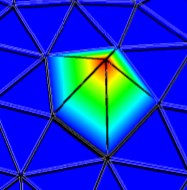
\includegraphics[scale=0.5]{elements_finis_P1}
\quad $\forall ({\ba},{\ba}') \in \Vh \times \Vh \quad \psi_{h,\ba}({\ba}')=\delta_{\ba}^{\ba'}.$
\end{definition}
\textcolor{red}{Idée naturelle: définir $\lambda_{1h}$, $\lambda_{2h}$ dans $\mathbb{X}_{0h}$ avec le produit scalaire $L^2$}

$\dps (\lambda_{1h},\psi_{h,\ba})_{\omega_{\ba}}=\mu_1 ({\bm \nabla} u_{1h},{\bm \nabla} \psi_{h,\ba})_{\omega_{\ba}}-(f_1,\psi_{h,\ba})_{\omega_{\ba}}$
\vspace{1 cm} 
$\dps (\lambda_{2h},\psi_{h,\ba})_{\omega_{\ba}}=-\mu_2 ({\bm \nabla} u_{
2h},{\bm \nabla} \psi_{h,\ba})_{\omega_{\ba}}+ (f_2,\psi_{h,\ba})_{\omega_{\ba}}$ 
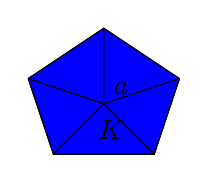
\begin{tikzpicture}[scale=0.32]
%%\draw[help lines] (0,0) grid (7,7);
\draw[fill=blue](0,4)--(3,6)--(6,4)--(5,1)--(1,1)--(0,4);
\draw(0,4)--(3,6)--(6,4)--(5,1)--(1,1)--(0,4);
\draw(1,1)--(3,3)--(5,1);
\draw (0,4)--(3,3)--(3,6);
\draw (3,3)--(6,4);
\draw[above right] (3,3) node {$a$};
\draw[above right] (2.4,1.2) node {$K$};
\end{tikzpicture}
%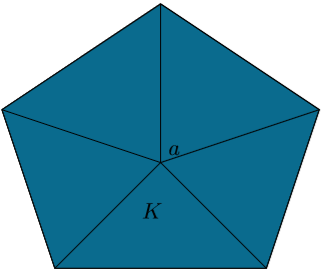
\includegraphics[scale=0.4]{patch}
\end{frame}

\begin{frame}
\begin{theorem}
$\lambda_{1h}=\lambda_{2h}=\lambda_h$.
\end{theorem}
\begin{remarque}

\includegraphics[scale=0.025]{attention}
\quad $\lambda_h$ n'est pas nécessairement positif. \textbf{Contre exemple:}
On a $\dps (\lambda_{h},\psi_{h,\ba})_{\omega_{\ba}} \geq 0 \nRightarrow \lambda_h \geq 0$. 
\begin{figure}

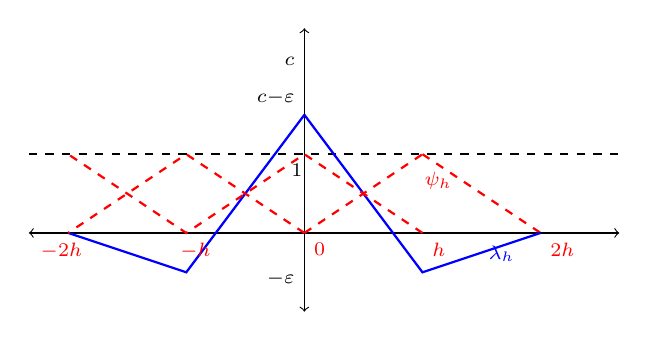
\begin{tikzpicture}[scale=1][xscale=2,yscale=2]
\draw [<->] (0,2.6) -- (0,0) -- (4,0);
\draw [<->] (0,-1) -- (0,0) -- (-3.5,0);
%%\draw [help lines] (-4,-4) grid (4,4);
\draw[black, dashed,  thick](-3.5,1)--(4,1);
\draw[below left][color=black] (0.1,1) node {$\scriptstyle \dps 1$};


\draw[below left][color=red] (2,0.9) node {$\scriptstyle \dps \psi_h$};

\draw[dashed,red,thick, domain=0:1.5] plot (\x, \x/1.5);
\draw[dashed,red,thick, domain=1.5:3] plot (\x, -\x/1.5+2);
\draw[below right][color=red] (1.5,0) node {$\scriptstyle \dps h$};
\draw[below right][color=red] (3,0) node {$\scriptstyle \dps 2h$};
\draw[below right][color=red] (0,0) node {$\scriptstyle \dps 0$};
\draw[above left][color=black] (0,2) node {$\scriptstyle \dps c$};
\draw[above left][color=black] (0,1.5) node {$\scriptstyle \dps c-\varepsilon$};
\draw[above left][color=black] (0,-0.8) node {$\scriptstyle -\dps \varepsilon$};
\draw[color=blue, thick] (0,1.5)--(1.5,-0.5)--(3,0);
\draw [above left][color=blue, thick] (2.8,-0.5) node {$\scriptstyle \dps \lambda_h$};
\draw [color=blue, thick](-3,0)--(-1.5,-0.5)--(0,1.5);
\draw [below right][color=red] (-1.7,0) node {$\scriptstyle \dps -h$};
\draw [below left][color=red] (-2.7,0) node {$\scriptstyle \dps -2h$};
\draw[dashed,color=red, thick](1.5,0)--(0,1)--(-1.5,0)--(-3,1);
\draw[dashed,color=red, thick](0,0)--(-1.5,1)--(-3,0);
\end{tikzpicture}

\end{figure}



%
%\begin{figure}
%\centering
%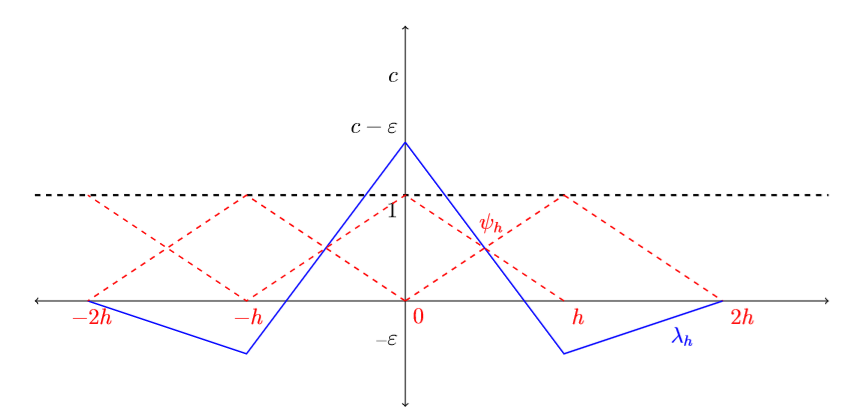
\includegraphics[scale=0.6]{contre_exemple}
%\end{figure}
\end{remarque}
\end{frame}
\begin{frame} 
\textcolor{red}{Alternative: mass lumping} 
\begin{equation*}
\dps (\lambda_{h},\psi_{h,\ba})_{\Omega} \approx \lambda_h({\ba}) ( \psi_{h,\ba},1)_{\omega_{\ba}}.
\end{equation*}
\begin{definition}
On définit $\lambda_{1h}$ et $\lambda_{2h}$ dans $\mathbb{X}_{0h}$ par $\forall \ba \in \Vhint$
\begin{equation}
\dps
\left\lbrace\begin{array}{llccc}
\dps \lambda_{1h}({\ba}) (\psi_{h,\ba},1)_{\omega_{\ba}}=\mu_1 (\nab u_{1h}, \nab \psi_{h,\ba})_{\Omega}-(f_1, \psi_{h,\bm a})_{\Omega}, \\\\
\dps \lambda_{2h}({\ba}) (\psi_{h,\ba},1)_{\omega_{\ba}}=-\mu_2 (\nab u_{2h}, \nab \psi_{h,\ba})_{\Omega}+(f_2, \psi_{h,\bm a})_{\Omega}.
\end{array}
\right.
\label{eq:555}
\end{equation}
\end{definition}
\begin{proposition}
Soit $(u_{1h},u_{2h})\in \Kgh$ solution de la formulation réduite \eqref{eq:probleme_variationnelle_discret_membrane}. Alors
\begin{equation}
\textcolor{red}{
\lambda_{1h}=\lambda_{2h} \geq 0}.
\end{equation}
\end{proposition}
\end{frame}
\begin{frame}
\begin{definition}
L'espace $\Lambda_h$ est défini par
\begin{align}
\Lambda_h=\left\{\lambda_h \in \mathbb{X}_{0h}; \hspace{0.15 cm} \lambda_h({\ba}) \geq 0 \quad \forall {\ba}\in \mathcal{V}_h^{\mathrm{int}}\right\}.
\label{eq: defcone}
\end{align}
\end{definition}

\textbf{FV pour le pb \eqref{eq:formulation_variationnelle_probleme_initial} :} trouver $(u_{1h},u_{2h},\lambda_h)\in {\mathbb{X}}_{gh} \times {\mathbb{X}}_{0h} \times \Lambda_h$ tq $\forall (v_{1h},v_{2h},\chi_h)\in {\mathbb{X}}_{0h} \times {\mathbb{X}}_{0h}\times \Lambda_h$
\begin{align*}
\dps
&\dps \sum_{i=1}^2 \mu_i  (\nab u_{ih},\nab v_{ih})_{\Omega}-\sum_{{\ba}\in \Vhint}[\lambda_h(v_{1h}-v_{2h})]({\ba})(\psi_{h,\ba},1)_{\omega_{\ba}}= \sum_{i=1}^2  (f_i,v_{ih})_{\Omega} \\
&\dps \sum_{{\ba}\in \Vhint}(\chi_h-\lambda_h)({\ba})(u_{1h}-u_{2h})({\ba}) \hspace{0.1 cm}\dps (\psi_{h,\ba},1)_{\omega_{\ba}}\geq 0.
%\label{eq:formulation_variationnelle_discret_probleme_complet}
\end{align*}


\end{frame}
\subsection{Analyse a posteriori}
\begin{frame}
\frametitle{Analyse a posteriori}
Un estimateur d'erreur a posteriori est donné par:
\begin{equation*}
|||u-u_h||| \leq \left\{\displaystyle\sum_{\substack{K \in\mathcal{T}_h}}\eta_K^2\right\}^{1/2} \quad \mbox{où \textcolor{red}{$\eta_K=\eta_K(u_h)$ ne dépend pas de $u$!}}
\end{equation*}
\begin{definition}
Soit ($u_1$,$u_2$) la solution continue de la formulation réduite \eqref{eq: formulation_variationnelle_probleme_reduit}. On définit les flux ${\bm{\sigma}}_1$ et ${\bm{\sigma}}_2$ par
\begin{equation}
{\bm{\sigma}}_1=-\mu_1 {\bm \nabla} u_1, \qquad {\bm{\sigma}}_2=-\mu_2{\bm \nabla} u_2 \quad.
\end{equation}
\end{definition}
\end{frame}
\begin{frame}
\begin{proposition}
\label{ref: proposition_5}
Soient $(f_1,f_2)\in (L^2(\Omega))^2$, $\lambda\in \Lambda$ et $g>0$. Soit ($u_1$,$ u_2$, $\lambda$) la solution continue définie dans  \eqref{eq:formulation_variationnelle_probleme_initial}.  Soient ${\bm{\sigma}}_1$ et ${\bm{\sigma}}_2$ les deux flux définis précédemment.
Alors 
\begin{equation}
({\bm{\sigma}}_1,{\bm{\sigma}}_2) \in (\textbf H(\div,\Omega))^2 \quad \mbox{et} \quad  \div {\bm{\sigma}}_1=f_1+\lambda \quad \mbox{et} \quad \div{\bm{\sigma}}_2=f_2-\lambda.
\end{equation}
\end{proposition}
\begin{remarque}
\begin{equation}
\nonumber -\mu_1{\bm{\nabla}} u_{1h} \notin  \textbf H(\div,\Omega), \quad -\mu_2{\bm{\nabla}} u_{2h} \notin \textbf H(\div,\Omega),
\end{equation}
\begin{equation}
\nonumber \div(-\mu_1{\bm{\nabla}} u_{1h}) \neq  f_1+\lambda_h,\quad
\div(-\mu_2{\bm{\nabla}} u_{2h}) \neq f_2-\lambda_h.
\end{equation}
\end{remarque}

%%\begin{equation}
%%\dps
%%\left\lbrace\begin{array}{llccc}
%%\dps{\bm{\sigma}}_{1h} \in \textbf H(\div,\Omega) \quad \mbox{tel que} \quad (\div {\bm{\sigma}}_{1h},1)_K=(f_1+\lambda_h,1)_K \quad \forall K \in \mathcal{T}_h, \\\\
%%\dps{\bm{\sigma}}_{2h} \in \textbf H(\div,\Omega) \quad\mbox{tel que} \quad (\div {\bm{\sigma}}_{2h},1)_K=(f_2-\lambda_h,1)_K \quad \forall K \in \mathcal{T}_h .
%\end{array}
%%\right.
%%\label{eq: 1.24}
%%\end{equation}
\end{frame}
\begin{frame}
\textbf{Semi norme d'énergie:}

$\forall {\bm v}=(v_1,v_2) \in (H^1(\Omega))^2 \quad |||{\bm v}|||=\dps \left\{\sum_{i=1}^2 \mu_i\left\|\nab v_i\right\|_{L^2(\Omega)}^2\right\}^{\frac{1}{2}}$.

\begin{theorem}
Soit $(f_1,f_2) \in (L^2(\Omega))^2$ et $g \geq 0$. Soient ${\bm u}$ solution faible du problème \eqref{eq: formulation_variationnelle_probleme_reduit} ,
${\bm u}_h\in \mathcal{K}_{gh}$ la solution approchée et $\lambda_h \in \Lambda_h$. Soient 
 ${\bm{\sigma}}_{1h}$ et ${\bm{\sigma}}_{2h}$ les flux équilibrés reconstruits. Alors, \vspace{-0.4 cm}
 \begin{equation}
 \textcolor{red}{\dps |||{\bm u}-{\bm u}_h|||\leq \left\{\sum_{K\in\Th}\left\{\sum_{i=1}^2(\etRKi+\etFKi)^2+\etCK\right\}\right\}^{\frac{1}{2}}}.
 \label{eq: a_posteriori_membrane} 
 \end{equation}

\vspace{-0.6 cm}
\begin{itemize}
\item[$\bullet$]${\small \dps \etFKi=\dps \left\|\dps \mu_i^{\frac{1}{2}} {\bm \nabla} u_{ih}+\mu_i^{-\frac{1}{2}} {\bm{\sigma}}_{ih}\right\|_{L^2(K)}}$,
\item[$\bullet$]$\dps \etRKi=\dps \frac{h_K}{\pi} \mu_i^{-\frac{1}{2}} \left\|f-\div {\bm{\sigma}}_{ih}-(-1)^i \lambda_h\right\|_{L^2(K)}$,
\item[$\bullet$]$\dps \etCK =\dps \left( u_{1h}-u_{2h},\lambda_h\right)_K$.
\end{itemize}

\end{theorem}
\end{frame}
\begin{frame}
\begin{corollary}
Sous les mêmes hypothèses et en notant $\dps \gamma=2 \max \left\{\mu_1^{\frac{1}{2}},\mu_2^{\frac{1}{2}}\right\}$ on a
$\textcolor{red}{\dps \left\|\lambda-\lambda_h\right\|_{H^{-1}(\Omega)}\leq \gamma\left\{\sum_{K\in\Th}\left\{\sum_{i=1}^2(\etRKi+\etFKi)^2+\etCK\right\}\right\}^{\frac{1}{2}}}$.
\end{corollary}

\includegraphics[scale=0.025]{attention} \quad
Dans le Théorème \eqref{eq: a_posteriori_membrane}  on a supposé que les flux équilibrés étaient reconstruits \ie
\begin{itemize}
\item[$\bullet$]$
\dps (f_1+\lambda_h-\div {\bm \sigma}_{1h},1)_K=0$,
\item[$\bullet$]$ 
\dps (f_2-\lambda_h-\div {\bm \sigma}_{2h},1)_K=0$.
\end{itemize}
\textcolor{red}{Comment reconstruire ces flux discrets rassemblant les propriétés des flux continus?}
\end{frame}
\begin{frame}
\textcolor{red}{Reconstruction des flux}
\begin{definition}
Soit $u_{1h}$ et $u_{2h}$ satisfaisant \eqref{eq:probleme_variationnelle_discret_membrane} et soit $\lambda_h$ donné par \eqref{eq: defcone}.
$\forall {\bm a} \in {\mathcal{V}}_h$, on définit $({\bm{\sigma}}_{1h}^{\bm a},{\bm{\sigma}}_{2h}^{\bm a}) \in ({\bf V}_h^{\bm a})^2$  et $(r_{1h}^{\bm a},r_{2h}^{\bm a})\in (Q_h^{\bm a})^2$ en résolvant un problème local par les éléments finis mixtes:
\begin{equation}
\left\lbrace\begin{array}{llccc}
\dps ({\bm{\sigma}}_{1h}^{\bm a},{\bm v}_{1h})_{{\omega}_{\bm a}}-(r_{1h}^{\bm a},\div \hspace{0.1 cm} {\bm v}_{1h})_{{\omega}_{\bm a}} &=& \dps -({\mathcal{\tau}}_{1h}^{\bm a},{\bm v}_{1h})_{\omega_{\bm a}} & \forall {\bm v}_{1h}\in {\bf V}_h^{\bm a}, \\
\dps (\div {\bm{\sigma}}_{1h}^{\bm a},q_{1h})_{\omega_{\bm a}}&=& \dps(g_{\mathrm{1}}^{\bm a},q_{1h})_{\omega_{\bm a}} & \forall  q_{1h} \in Q_h^{\bm a},\\
\dps ({\bm{\sigma}}_{2h}^{\bm a},{\bm v}_{2h})_{\omega_{\bm a}}-(r_{2h}^{\bm a},\div {\bm v}_{2h})_{\omega_{\bm a}} &=& \dps -({\mathcal{\tau}}_{2h}^a,{\bm v}_{2h})_{\omega_{\bm a}} &\forall {\bm v}_{2h} \in {\bf V}_h^{\bm a},\\
\dps(\div {\bm{\sigma}}_{2h}^{\bm a},q_{2h})_{\omega_{\bm a}}&=&\dps(g_{\mathrm{2}}^{\bm a},q_{2h})_{\omega_{\bm a}} & \forall q_{2h} \in Q_h^{\bm a}.
\end{array}
\right.
\label{eq:reconstruction_flux_raviart_thomas}
\end{equation}
\end{definition}
\begin{definition}
%%On définit l'espace de Raviart--Thomas--Nédélec
%$\textbf{RT}_1(\Omega)=\left\{{\bm v}_h \in \textbf H(\div,\Omega), {{\bm v}_h}_{|K} \in \textbf{RT}_1(K) \hspace{0.15 cm} \forall K \in \mathcal{T}_h\right\}$
%où 
$\textbf{RT}_1(K)=({\mathbb{P}}_1)^d + {\bf x} {\mathbb{P}}_1(K)$.
\end{definition}
\end{frame}
\begin{frame}
\begin{itemize}
\item[$\bullet$]Pour ${\bm a} \in {\mathcal{V}}_h^{int}$
\end{itemize}
${\bf V}_h^{\bm a}=\left\{{\bm v}_h \in \textbf H(\div,\omega_{\bm a}), {{\bm v}_h}_{|K}\in \textbf{RT}_1(K), \hspace{0.1 cm} {\bm v}_h\cdot {\bf n}_{\omega_{\bm a}}=0 \hspace{0.1 cm} \mbox{sur} \hspace{0.1 cm} \partial \omega_{\bm a} \right\},$\\
$Q_h^{\bm a}=\left\{q_h \in L^2(\omega_{\bm a}),\hspace{0.2 cm} {q_h}_{|K} \in {\mathbb{P}}_1(K),\hspace{0.2 cm} (q_h,1)_{\omega_{\bm a}}=0\right\}.$
\\
\begin{itemize}
\item[$\bullet$]Pour ${\bm a} \in {\mathcal{V}}_h^{ext}$
\end{itemize}
${\bf V}_h^{\bm a}=\left\{{\bm v}_h \in \textbf H(\div,\omega_{\bm a}), {{\bm v}_h}_{|K}\in \textbf{RT}_1(K),\hspace{0.1 cm} {\bm v}_h\cdot {\bf n_{\omega_{\bm a}}}=0 \hspace{0.1 cm} \mbox{sur} \hspace{0.1 cm} \partial \omega_{\bm a}\backslash \partial\Omega\right\},$\\
$Q_h^{\bf a}=\left\{q_h \in L^2(\omega_{\bm a}), \hspace{0.2 cm} {q_h}_{|K} \in {\mathbb{P}}_1(K) \right\}.$
\\
Enfin,
\begin{itemize}
\item[$\bullet$] $\dps g_{\mathrm{1}}^{\bm a}=\psi_{\bm a} f_1-\mu_1 {\bm \nabla} \psi_{\bm a} \cdot {\bm \nabla}  {u_{1h}}+\lambda_h \psi_{\bm a}$, 
\label{eq: fonction_ g_1^a}
\\
\item[$\bullet$] $\dps g_{\mathrm{2}}^{\bm a} = \psi_{\bm a} f_2-\mu_2 {\bm \nabla} \psi_{\bm a} \cdot {\bm \nabla}  u_{2h}-\lambda_h \psi_{\bm a}$,
\label{eq: fonction_g_2^a}\\
\item[$\bullet$] ${\bm{\mathcal{\tau}}}_{1h}^{\bm a}= \psi_{\bm a} {\bm \nabla} u_{1h}$,\quad ${\bm{\mathcal{\tau}}}_{2h}^{\bm a}= \psi_{\bm a} {\bm \nabla} u_{2h}$.\\
\item[$\bullet$] $\dps {\bm{\sigma}}_{1h}=\sum_{{\bm a}\in {\mathcal{V}}_h} {\bm{\sigma}}_{1h}^{\bm a}$, \quad  $\dps {\bm {\sigma}}_{2h}= \sum_{{\bm a}\in {\mathcal{V}}_h} {\bm{\sigma}}_{2h}^{\bm a}$. 
\label{ref: fonction_sigma2h}
\end{itemize}
\end{frame}
\begin{frame}

\textcolor{red}{Avantage de la reconstruction des flux par cette méthode:}
\begin{itemize}
\item[$\bullet$]Les flux reconstruits appartiennent à l'espace $\textbf H(\div,\Omega)$.
\item[$\bullet$] Les flux sont localement conservatifs.
\end{itemize}
\begin{theorem}
Les flux $\dps {\bm \sigma}_{1h}$ et ${\bm \sigma}_{2h}$ reconstruits 
%dans \eqref{eq:reconstruction_flux_raviart_thomas} 
par la méthode des éléments finis mixtes vérifient
$\dps ({\bm \sigma}_{1h},{\bm \sigma}_{2h}) \in \textbf H(\div,\Omega) \times \textbf H(\div,\Omega)$ et $\forall (q_{1h},q_{2h})\in Q_h(K) \times Q_h(K) $
\begin{equation}
\dps
\left\lbrace\begin{array}{ll}
\dps (f_1+\lambda_h-\div {\bm \sigma}_{1h},q_{1h})_K=0, \\\\
\dps (f_2-\lambda_h-\div {\bm \sigma}_{2h},q_{2h})_K=0,
\end{array}
\right.
\label{eq: reconstruction_flux}
\end{equation}
avec $Q_h(K)=\left\{q_h \in L^2(K), \hspace{0.2 cm} {q_h}_{|K} \in {\mathbb{P}}_1(K)\right\}$.
\end{theorem}
\end{frame}
\begin{frame}
\textcolor{red}{formule explicite pour les flux ${\bm \sigma}_{1h}$ et ${\bm \sigma}_{2h}$}
La formulation duale mixte   \eqref{eq:reconstruction_flux_raviart_thomas}
est équivalente à la formulation duale:
Trouver ${\bm{\sigma}}_{1h}^{\ba} \in {\bf V}_h^{\ba}$ et ${\bm{\sigma}}_{2h}^{\ba} \in {\bf V}_h^{\ba}$ avec $\div {\bm{\sigma}}_{1h}^{\ba}={\bm \Pi}_{Q_h^{\bm a}}\guna$ et $\div {\bm{\sigma}}_{2h}^{\ba}={\bm \Pi}_{Q_h^{\bm a}} \gdeuxa$ tel que
\begin{equation}
\dps
\left\lbrace\begin{array}{ll}
({\bm{\sigma}}_{1h}^{\ba},{\bm v}_{1h})_{\oma}=-(\tauunha,{\bm v}_{1h})_{\oma}, \quad \forall {\bm v}_{1h} \in  {\bf V}_h^{\ba} \quad \mbox{avec} \quad \div {\bm v}_{1h}=0
\\
({\bm{\sigma}}_{2h}^{\ba},{\bm v}_{2h})_{\oma}=-(\taudeuxha,{\bm v}_{2h})_{\oma}, \quad \forall {\bm v}_{2h} \in  {\bf V}_h^{\ba} \quad \mbox{avec} \quad \div {\bm v}_{2h}=0.
\label{eq: system_dual_2}
\end{array}
\right.
\end{equation}
Le système précédent coïncide avec un problème de minimisation sous contraintes:
\begin{equation}
{\bm{\sigma}}_{1h}^{\ba}=\argmin\limits_{\substack{{\bm v}_{1h} \in {\bf V}_h^{\ba},\\ \div {\bm v}_{1h}= 
{\dps {\bm \Pi}}_{Q_h^{\ba}}\guna}} \frac{1}{2}\left\|\tauunha+{\bm v}_{1h}\right\|^2_{\oma}, 
\label{eq: minimisation_system_dual_1}
\end{equation}
\begin{equation}
{\bm{\sigma}}_{2h}^{\ba}=\argmin\limits_{\substack{{\bm v}_{2h} \in {\bf V}_h^{\ba},\\ \div {\bm v}_{2h}= 
{\dps {\bm \Pi}}_{Q_h^{\ba}}g_{\mathrm{2}}^{\ba}}}  \frac{1}{2}\left\|\taudeuxha+{\bm v}_{2h}\right\|^2_{\oma}. 
\label{eq: minimisation_system_dual_2}
\end{equation}
\end{frame}
%\subsection{Efficacité Locale}
%\begin{frame}
%\frametitle{Efficacité locale}
%\end{frame}
\subsection{Résolution}
\begin{frame}
\frametitle{Résolution}
\begin{align}
\dps
&\nonumber \dps \sum_{i=1}^2 \mu_i  (\nab u_{ih},\nab v_{ih})_{\Omega}-\sum_{{\ba}\in \Vhint}[\lambda_h(v_{1h}-v_{2h})]({\ba})(\psi_{h,\ba},1)_{\omega_{\ba}}= \sum_{i=1}^2  (f_i,v_{ih})_{\Omega} \\
&\dps \sum_{{\ba}\in \Vhint}(\chi_h-\lambda_h)({\ba})(u_{1h}-u_{2h})({\ba})\dps (\psi_{h,\ba},1)_{\omega_{\ba}}\geq 0.\label{eq:formulation_variationnelle_discret_probleme_complet}
\end{align}

%${\mathbb{X}}_{0h}$ et $\Lambda_h$ sont des espaces vectoriels de dimension fini.
$N_h=\dim \mathbb{X}_{0h}$ et soit $(\psi_{h,\ba})_{\ba \in \Vhint}$ une base de $\mathbb{X}_{0h}$.\\
$\mathbb{X}_{gh}$ est un espace affine: $\mathbb{X}_{gh}=\mathbb{X}_{0h}+\tilde{g}_h$ avec $\tilde{g_h}$ un recouvrement appartenant à l'espace ${\mathbb{X}}_h$ tel que $\tilde{g_h}_{|\partial\Omega}=g$.
\begin{itemize}
\item[$\bullet$]$\dps u_{2h}=\sum_{{\ba}\in \Vhint} u_{2h}({\ba})\psi_{h,{\ba}}$,
\item[$\bullet$]$\dps u_{1h}=u_{1h}^0+\tilde{g_h}=\sum_{{\ba}\in\Vhint} u_{1h}^0({\ba})\psi_{h,{\ba}}+\tilde{g_h}$
\end{itemize}

\end{frame}
\begin{frame}
\textcolor{red}{$v_{1h}=0$ et $v_{2h}=\psi_{h,\ba'}$ dans la 1ère ligne de \eqref{eq:formulation_variationnelle_discret_probleme_complet} puis $v_{2h}=0$ et $v_{1h}=\psi_{h,\ba'}$:}
\begin{align*}
\dps
&\mu_1 \dps \sum_{{\ba}\in\Vhint} u_{1h}^0({\ba}) \left(\nab \psi_{h,{\ba}},\nab \psi_{h,{\ba}'}\right)_{\Omega}-\lambda_h({{\ba}'}) \left(\psi_{h,{\ba}'},1\right)_{\omega_{{\ba}'}}\\
&=\left(f_1 \psi_{h,{\ba}'}-\mu_1\nab \tilde{g_h} \cdot \nab \psi_{h,{\ba}'},1\right)_{\Omega},\\\\
&\mu_2 \dps \sum_{{\ba}\in\Vhint} u_{2h}({\ba}) \left(\nab \psi_{h,{\ba}}, \nab \psi_{h,{\ba}'}\right)_{\Omega}+\lambda_h({{\ba}'}) \left(\psi_{h,{\ba}'},1\right)_{\omega_{{\ba}'}}=\left(f_2,\psi_{h,{\ba}'}\right)_{\Omega}.
\end{align*}
Le système précédent s'écrit sous forme matricielle: $A\Xh=F$ où
\begin{equation}
A=
\begin{pmatrix}
\mu_1 {\Huge A_1} & {\Huge 0} & {\Huge -B}\\\\
{\Huge 0} &\mu_2 {\Huge A_1} &{\Huge B} 
\end{pmatrix}\in \mathcal{M}_{2N_h,3N_h}(\mathbb{R})
\label{eq:matrice_rigidité}
\end{equation}
avec 
\end{frame}
\begin{frame}
\begin{equation}
A_1=
\begin{pmatrix}
\dps \left(\nab \psi_{{{\ba}_1}}, \nab \psi_{{{\ba}_1}}\right)_{\Omega}  &\ldots& \dps \left(\nab \psi_{{{\ba}_{N_h}}},\nab \psi_{{{\ba}_1}}\right)_{\Omega}\\\\
\vdots& \ddots&\vdots\\\\
\dps \left(\nab \psi_{{{\ba}_1}},\nab \psi_{{{\ba}_{N_h}}}\right)_{\Omega}  &\ldots& \dps \left(\nab \psi_{{{\ba}_{N_h}}},\nab \psi_{{{\ba}_{N_h}}}\right)_{\Omega}
\end{pmatrix}
\in \mathcal{M}_{N_h,N_h}(\R)
\label{eq:matrice_A1}
\end{equation}
\begin{equation}
B=
\begin{pmatrix}
\dps \left(\psi_{{\ba}_1},1\right)_{\omega_{{\ba}_1}}& 0 & \ldots & 0\\
0& \ddots & 0 &0\\
\vdots& &\ddots& \vdots\\
\vdots&  &  & 0\\
0&\ldots& 0&\dps\left(\psi_{{\ba}_{N_h}},1\right)_{\omega_{{\ba}_{N_h}}}
\end{pmatrix}\in \mathcal{M}_{N_h,N_h}(\R)
\label{eq:matrice_de_masse}
\end{equation}
\end{frame}
\begin{frame}
\begin{equation}
F=
\begin{pmatrix}
\dps  \left(f_1 \psi_{{\ba}_1}-\mu_1\nab \tilde{g_h} \cdot \nab \psi_{{\ba}_1},1\right)_{\Omega}\\
\vdots\\
\dps \left(f_1 \psi_{{\ba}_{N_h}}-\mu_1\nab \tilde{g_h} \cdot \nab \psi_{{\ba}_{N_h}},1\right)
\\
\dps \left(f_2,\psi_{{\ba}_1}\right)_{\Omega}\\
\vdots\\
\dps \left(f_2,\psi_{{\ba}_{N_h}}\right)_{\Omega}
\end{pmatrix}
\in \mathcal{M}_{2N_h,N_h}(\R)
\label{eq: definition_matrice_F}
\end{equation}
Le vecteur des inconnues $\Xh \in \mathcal{M}_{3N_h,1}(\R)$ est défini par
\\
\begin{equation*}
\Xh^T=\left(u_{1h}^0({{\ba}_1}) \ldots u_{1h}^0({{\ba}_{N_h}}),u_{2h}({{\ba}_1}) \ldots u_{2h}({{\ba}_{N_h}}),\lambda_h({{\ba}_1}) \ldots \lambda_h({{\ba}_{N_h}})\right).
%\label{eq: vecteur_X}
\end{equation*}
%\begin{remarque}
%$A$ n'est pas carré on ne peut pas résoudre le système.
%\end{remarque}
\end{frame}
\begin{frame}
\textcolor{red}{Idée: Simplifier la deuxième ligne de \eqref{eq:formulation_variationnelle_discret_probleme_complet}.}
\begin{theorem}
Soit $u_h\in\Kgh$ solution de \eqref{eq:probleme_variationnelle_discret_membrane} et soit $\lambda_h\in\Lambda_h$. Les trois expressions suivantes sont équivalentes $\forall \ba \in \Vh$
\begin{align}
& \dps \forall \chi_h \in \Lambda_h \dps \sum_{{\ba}\in \Vhint}(\chi_h-\lambda_h)({\ba})(u_{1h}-u_{2h})({\ba})(\psi_{h,\ba},1)_{\omega_{\ba}}\geq 0 
\label{eq:preuve_equivalence_part_1}
\\
& (u_{1h}-u_{2h})(\ba) \geq 0, \hspace{0.15 cm} \lambda_h(\ba) \geq 0, \hspace{0.15 cm} [\lambda_h (u_{1h}-u_{2h})](\ba)=0
\label{eq:preuve_equivalence_part_2}
\\
& \textcolor{red}{\min(u_{1h}-u_{2h},\lambda_h)=0}.
\label{eq:preuve_equivalence_part_3 }
\end{align}
\textcolor{red}{Preuve:}
\begin{itemize}
\item $\eqref{eq:preuve_equivalence_part_1}
\Rightarrow \eqref{eq:preuve_equivalence_part_2}$:
On remplace $\chi_h$ par $0\in \Lambda_h$ et $\chi_h$ par $2\lambda_h\in\Lambda_h$.
\item $\eqref{eq:preuve_equivalence_part_2} \Rightarrow \eqref{eq:preuve_equivalence_part_1}$: On utilise $[\lambda_h (u_{1h}-u_{2h})](\ba)=0$.
\item $ \eqref{eq:preuve_equivalence_part_2} \Leftrightarrow \eqref {eq:preuve_equivalence_part_3 }$: évident
\end{itemize}

\end{theorem}
\end{frame}
\begin{frame}
\begin{itemize}
\item[$\bullet$]
$\begin{array}{ccccc}
\textbf{H} & : &\mathcal{M}_{3N_h,1}(\R) & \to & \mathcal{M}_{2N_h,1}(\R) \\\\
 & & \Xh
 & \longmapsto & A\Xh-F.\\\\
\end{array}$

\item[$\bullet$]$
\begin{array}{ccccc}
\textbf{K} & : & \mathcal{M}_{3 N_h,1}(\R) & \to &\mathcal{M}_{N_h,1}(\R) \\\\
 & & \Xh
 & \longmapsto & \left(\begin{array}{c}
u_{1h}^0({{\ba}_1})-u_{2h}({{\ba}_1})+\tilde{g_h}\\
\vdots\\
\dps u_{1h}^0({{\ba}_{N_h}})-u_{2h}({{\ba}_{N_h}})+\tilde{g_h}\\ 
\end{array}\right).
\end{array}$
\item[$\bullet$]$
\begin{array}{ccccc}
\textbf{G} & : &  \mathcal{M}_{3 N_h,1}(\R) & \to & \mathcal{M}_{N_h,1}(\R) \\\\
& & {\Xh} & \longmapsto & \left(\begin{array}{c}
\lambda_h({{\ba}_1})\\
\vdots\\
\lambda_h({{\ba}_{N_h}})\\ 
\end{array}\right)
\end{array}$.
\end{itemize}
\end{frame}
\begin{frame}
Le problème \eqref{eq:formulation_variationnelle_discret_probleme_complet} peut se réécrire sous forme compacte:
\begin{align}
&{\bf H}(\Xh)=0,
\label{eq: pp}\\
&C(\Xh)=\min({\bf K}(\Xh),{\bf G}(\Xh))=0,
\label{eq: ppp}
\end{align}
ou 

\begin{equation}
\boxed{{\bm \Pi}(\Xh)=0}.
\end{equation}

\includegraphics[scale=0.025]{attention} \quad \textcolor{red}{La fonction $C$ n'est pas différentiable donc l'algorithme de Newton classique ne marche pas. On utilise l'algorithme de Newton--min.}
\end{frame}
\subsection{Algorithme Newton--min}
\begin{frame}
\frametitle{Algorithme Newton--min}
\textbf{Initialisation} ${\Xh^0} \in {\mathbb{R}}^{3N_h}$.\\
Pour $k\in\mathbb{N}$ on construit deux ensembles d'indices complémentaires: \begin{equation}
\left\lbrace\begin{array}{rclrl}
B^k &=&\{\mathrm{i}:{\bf G_i}(\Xh^k)\leq {\bf F_i}(\Xh^k)\} \subset \{1 \ldots N_h \},\\
I^k &=&\{\mathrm{i}:{\bf G_i}({\Xh^k})>{\bf F_i}({\Xh^k})\}\subset\{1\ldots
N_h\}.
\end{array}
\right.
\end{equation}
${\Xh^k}$ est solution de
\begin{equation}
\left\lbrace\begin{array}{rclrl}
{\bf H}(\Xh^k)+{\bf H'}(\Xh^k)(\Xh^{k+1}-\Xh^k)=0,\\
{\bm C}(\Xh^k)+{\bf J}_{\Xh^k}(\Xh^{k+1}-\Xh^k)=0.
\end{array}
\right.
\end{equation}
Ici, ${\bf J}_{\Xh^k}$ est la pseudo-jacobienne de ${\bm C}$ en $\Xh^k$ définie par
\begin{equation}
({\bf J}_{\Xh^k})_i=
\left\lbrace\begin{array}{rclrl}
{\bf G}_{\mathrm{i}}'(\Xh^k)\quad \mbox{si} \quad \mathrm{i}\in B^k,\\
{\bf F}_{\mathrm{i}}'(\Xh^k) \quad \mbox{si} \quad \mathrm{i}\in I^k.
\end{array}
\right.
\end{equation}
\textbf{Critère d'arrêt:} $\left\|{\bm \Pi}(\Xh^{k+1})\right\|_2\leq \varepsilon$. %alors $\Xh^{k+1}$
% bonne approximation du zéro.
\end{frame}
%\begin{frame}
%\begin{algorithmic}
%\STATE $\mbox{\textbf {Initialisation}}: \Xh^0 \in {\R}^{3N_h} \quad \mbox{et on pose} \quad k=0$
%\WHILE{$\left\|{\bf \Pi}(\Xh^k)\right\|>\varepsilon$}
%\STATE $\mbox{Pour $k\in\mathbb{N}$ on construit deux ensembles d'indices complémentaires:}$ 
%
%%$%%\left\lbrace\begin{array}{rclrl}
%%{\bf G}_{\mathrm{i}}'(\Xh^k)$ \quad \mbox{si} \quad $\mathrm{i}\in B^k,\\
%%{\bf F}_{\mathrm{i}}'(\Xh^k)$ \quad \mbox{si} \quad $\mathrm{i}\in I^k.
%%\end{array}
%%\right.
%%$}$
%\end{algorithmic}
%\end{frame}
%\section{Écoulement diphasique liquide--gaz  comme un problème de complémentarité non linéaire en milieu poreux}
%%\title{Écoulement diphasique liquide--gaz  comme un problème de complémentarité non linéaire en milieu poreux}
%\label{ref: chap2}
%\subsection{Etude préliminaire}
%\begin{frame}
%\frametitle{Écoulement diphasique liquide--gaz avec échange entre les phases comme un problème de complémentarité non linéaire en milieu poreux}
%\vspace{-0.5 cm}
%\begin{equation}
%\dps
%\left\lbrace\begin{array}{llccc}
%\dps \frac{\partial}{\partial t} (\phi \gamma \textcolor{red}{S_{\mathrm{l}}})+\div(\gamma {\bf q_l}- {\bf J}_{\bm {\mathrm{h}}}^{\bf l}) = Q_{\mathrm{\textcolor{blue}{w}}}, \\
%\dps\frac{\partial}{\partial t} \left[\phi \beta_{\mathrm{l}} \textcolor{red}{\chi_{\mathrm{h}}^{\mathrm{l}}} \textcolor{red}{S_{\mathrm{l}}}+\phi \beta_g P_g S_g\right]+\div\left[\rho_{\mathrm{h}}^{\mathrm{l}} \textbf q_{\textbf l}+ \beta_g P_g {\bf q}_{\bm g}+ {\bf J}_{\bm {\mathrm{h}}}^{\bf l} \right]=Q_{\mathrm{{\textcolor{blue}{h}}}},\\
%1-\textcolor{red}{S_{\mathrm{l}}} \geq 0, \hspace{0.15 cm}
%H(\textcolor{red}{P_{\mathrm{l}}}+P_c(\textcolor{red}{S_{\mathrm{l}}}))-\beta_{\mathrm{l}} \textcolor{red}{\chi_{\mathrm{h}}^{\mathrm{l}}} \geq 0,\\
%\dps (1-\textcolor{red}{S_{\mathrm{l}}})\left[H(\textcolor{red}{P_{\mathrm{l}}}+P_c(\textcolor{red}{S_{\mathrm{l}}}))-\beta_{\mathrm{l}} \textcolor{red}{\chi_{\mathrm{h}}^{\mathrm{l}}}\right]=0.
%\end{array}
%\right.
%\label{systeme_edp_depart}
%\end{equation}
%\vspace{-0.55 cm}
%\begin{itemize}
%\item[$\bullet$]
%$\chi_{\mathrm{d}}^i=\frac{C_{\mathrm{d}}^i}{C_i}$, \quad \fbox{$S_l+S_g=1$}
%\item[$\bullet$]
%$P_c(S_l)=P_g-P_l$, \quad \fbox{$H P_g=\rho_{\mathrm{h}}^{\mathrm{l}}$: Loi de Henry}
%\item[$\bullet$] 
%${\bf q}_{\bm i}=-K \frac{\displaystyle k_{ri}(S_i)}{ \displaystyle \mu_i} ({\bm \nabla} P_i-\rho_i g {\bm\nabla} z)$: vitesse de Darcy
%\item[$\bullet$]${\bf J}_{\bm {\mathrm{d}}}^{\bm i}=- M^{\mathrm{d}} S_i C_i D_{\mathrm{d}}^i {\bm \nabla} \chi_{\mathrm{d}}^i$: Loi de Fick
%\end{itemize}
%\end{frame}
%\subsection{Discrétisation}
%\begin{frame}
%\frametitle{Discrétisation}
%\begin{itemize}
%\item[$\bullet$] discrétisation en temps: \textcolor{red}{schéma d'Euler implicite} $\{t^n\}_{0\leq n\leq N_t}$ une suite croissante de temps $\geq 0$, tel que $t^0=0$, $t^{N_t}=T$ et $I_n=(t^{n-1},t^n]$ et le pas de temps $\tau^n=t^n-t^{n-1}=\Delta t$. 
%\item[$\bullet$] discrétisation en espace: \textcolor{red}{méthode des volumes finis} On discrétise l'intervalle $(0,L)$ en $\Nx$ intervalles de longueurs $h$.
%\end{itemize}
%\vspace{-1cm}
%\begin{figure}[htdp]
%\centering
%\begin{picture}(320,60)(0,0)
%\thicklines
%\put(0,15){\line(320,0){320}}
%\put(0,10){\red{\line(0,10){10}}}
%\put(0,0){\makebox(0,0){\small \red{$x_{1/2}$}}}
%\put(0,15){\black{\circle*{6}}}
%\put(40,10){\red{\line(0,10){10}}}
%\put(40,0){\makebox(0,0){\small \red{$x_{3/2}$}}}
%\put(20,15){\blue{\circle*{6}}}
%\put(20,30){\makebox(0,0){\small  \blue{$j=1$}}}
%\put(80,10){\red{\line(0,10){10}}}
%\put(80,0){\makebox(0,0){\small \red{$x_{5/2}$}}}
%\put(60,15){\blue{\circle*{6}}}
%\put(60,30){\makebox(0,0){\small  \blue{$j=2$}}}
%\put(120,30){\makebox(0,0){\small \blue{$\cdots$}}}
%\put(120,0){\makebox(0,0){\small \red{$\cdots$}}}
%\put(180,30){\makebox(0,0){\small \blue{$j$}}}
%\put(180,15){\blue{\circle*{6}}}
%\put(160,10){\red{\line(0,10){10}}}
%\put(160,0){\makebox(0,0){\red{\small $x_{j-1/2}$}}}
%\put(200,10){\red{\line(0,10){10}}}
%\put(200,0){\makebox(0,0){\red{\small $x_{j+1/2}$}}}
%\put(240,30){\makebox(0,0){\small \blue{$\cdots$}}}
%\put(240,0){\makebox(0,0){\small \red{$\cdots$}}}
%\put(280,0){\makebox(0,0){\small \red{$x_{(N_x-1/2)}$}}}
%\put(280,10){\red{\line(0,10){10}}}
%\put(300,15){\blue{\circle*{6}}}
%\put(300,30){\makebox(0,0){\small \blue{$j=N_x$}}}
%\put(317,0){\makebox(0,0){\small \red{$x_{(N_x+1/2)}$}}}
%\put(320,10){\red{\line(0,10){10}}}
%\put(320,15){\black{\circle*{6}}}
%\end{picture}
%\end{figure}
%${\bm y}^n$, ($n=1 \ldots \Nt$): vecteur des inconnues discrétisées: 
%$({\bm y^T})^n=\left(S_{\mathrm{l},1}^n \ldots S_{\mathrm{l},\Nx}^n,P_{\mathrm{l},1}^n \ldots P_{\mathrm{l},N_x}^n,(\chi_{\mathrm{h}}^{\mathrm{l}})_1^n \ldots (\chi_{\mathrm{h}}^{\mathrm{l}})_{N_x}^n\right)
%$.
%\end{frame}
%%%
%%%\begin{frame}
%%%\begin{equation}
%%%%\dps
%%%\left\lbrace\begin{array}{llccc}
%%%\dps{\bf H}_{{\bm j},{\bf w}}({\bm y^{n+1}}) = \phi \gamma \frac{S_{\mathrm{l},j}^{n+1}-S_{\mathrm{l},j}^n}{\Delta t}\\
%%%+\dps \frac{\gamma(\textbf q_{\textbf l,j+1/2}^{n+1}-\textbf q_{\textbf l,j-1/2}^{n+1})-(({\bf J}_{\bm {\mathrm{h}}}^{\bm{\mathrm{l}}})_{j+1/2}^{n+1}-({\bf J}_{\bm {\mathrm{h}}}^{\bm{\mathrm{l}}})_{j-1/2}^{n+1})}{h}-Q_{\mathrm{w},h}^{n+1}\\
%%%(\mbox{pour l'eau}) \quad \forall j \in\{1 \ldots,\Nx\},\\\\
%%%\dps{\bf H}_{{\bm j},{\bf h}}({\bm y^{n+1}})= 
%%%\\
%%%\dps \phi \left[\frac{\beta_{\mathrm{l}}(S_{\mathrm{l},j}^{n+1} (\chi_{\mathrm{h}}^{\mathrm{l}})_j^{n+1}-S_{\mathrm{l},j}^n (\chi_{\mathrm{h}}^{\mathrm{l}})_j^{n+1}}{\Delta t}+\dps \frac{\rho_{g,j}^{n+1} (1-S_{\mathrm{l},j}^{n+1})-\dps \rho_{g,j}^n (1-S_{\mathrm{l},j}^n)}{\Delta t}\right]\\+\displaystyle \beta_{\mathrm{l}} \frac{\textbf q_{\textbf l,j+1/2}^{n+1} (\chi_{\mathrm{h}}^{\mathrm{l}})_{j+1}^{n+1}- \textbf q_{\textbf l,j-1/2}^{n+1} (\chi_{\mathrm{h}}^{\mathrm{l}})_j^{n+1}}{h}
%%%+
%%%\\
%%%\dps\frac{\rho_{g,j+1/2}^{n+1} {\bf q}_{{\bm g},j+1/2}^{n+1}-\rho_{g,j-1/2}^{n+1} {\bf q}_{{\bm g},j-1/2}^{n+1}}{h}
%%%+\dps\frac{({\bf J}_{\bm {\mathrm{h}}}^{\bm{\mathrm{l}}})_{j+1/2}^{n+1}-({\bf J}_{\bm {\mathrm{h}}}^{\bm{\mathrm{l}}})_{j-1/2}^{n+1}}{h}-\dps Q_{j,\mathrm{h}}^{n+1}\\
%%%(\mbox{pour l'hydrogène}) \quad \forall j\in\{1 \ldots \Nx\}.
%%%\end{array}
%%%\right.
%%%\label{eq: systeme_Hj}
%%%\end{equation}
%%%\end{frame}
%\subsection{Méthode de résolution}
%\begin{frame}
%\frametitle{Méthode de résolution}
%$\begin{array}{ccccc}
%\dps{\bf H}_{{\bm j},{\bf z}} & : & \mathbb{R}^{3N_x} & \to & \mathbb{R}^{N_x} \\
% & & {\bm y^{n+1}}
% & \longmapsto & \dps{\bf H}_{{\bm j},{\bf z}}({\bm y^{n+1}}) \quad z\in\left\{w,h\right\}.
%\end{array}$
%\\
%$\begin{array}{ccccc}
%\textbf{F} & : & \mathbb{R}^{3N_x} & \to & \mathbb{R}^{N_x} \\
% & & {\bm y^n}
% & \longmapsto & \left(\begin{array}{c}
%1-S_{\mathrm{l},1}^n\\
%1-S_{\mathrm{l},2}^n \\
%\vdots\\
%1-S_{\mathrm{l},N_x}^n\\ 
%\end{array}\right)
%\end{array}$.
%\vspace{0.4 cm}
%$\begin{array}{ccccc}
%\textbf{G} & : & \matR^{3\Nx} & \to & \matR^{\Nx} \\
% & & {\bm y^n} & \longmapsto & \left(\begin{array}{c}
% H(P_{\mathrm{l},1}^n+P_c(S_{\mathrm{l},1}^n))-\beta_{\mathrm{l}} (\chi_{\mathrm{h}}^{\mathrm{l}})_1^n\\
%H(P_{\mathrm{l},2}^n+P_c(S_{\mathrm{l},2}^n))-\beta_{\mathrm{l}} (\chi_{\mathrm{h}}^{\mathrm{l}})_2^n\\
%\vdots\\
% H(P_{\mathrm{l},N_x}^n+P_c(S_{\mathrm{l},N_x}^n))-\beta_{\mathrm{l}} (\chi_{\mathrm{h}}^{\mathrm{l}})_{N_x}^n\\ 
%\end{array}\right)
%\end{array}$
%\end{frame}
%\begin{frame}
%A chaque pas de temps le problème peut s'écrire sous la forme compacte suivante:
%\begin{align}
% \nonumber {\bf H}({\bm y})=0, (\mbox{\textcolor{red}{2n équations}})\\
%{\bf F}({\bm y})\top {\bf G}({\bm y}) \quad \mbox{et} \quad {{\bf F}({\bm y})} \geq 0 \quad \mbox{et} \quad {\bf G}({\bm y}) \geq 0,
%\label{eq: pb_complementarite_contraintes}
%\end{align}
%\textcolor{red}{Problème: $2n$ équations pour $3n$ inconnues}
%\\
%On introduit la fonction ${\bm \zeta}$ définie par:
%\begin{equation}
%\underbrace{\bm{\zeta{\bm(y)}}=\min({\bf F}({\bm y}),{\bf G}({\bm y}))}_{\mbox{non différentiable}}. \quad \textcolor{red}{\mbox {$n$ équations}}
%\end{equation}
%Les contraintes de complémentarités \eqref{eq: pb_complementarite_contraintes} sont équivalentes à résoudre ${\bm {\zeta{\bm (y)}}}=0$.
%On veut résoudre:
%\begin{equation}
%{\bm \Pi}({\bm y})= \left( \begin{array}{c}
% {\bf H}({\bm y})\\
%{\bm \zeta}({\bm y})\\
%\end{array} \right)=0.
%\end{equation}
%\end{frame}
%%\subsection{Algorithme Newton--min}
%%\begin{frame}
%%\frametitle{Algorithme Newton--min}
%%\begin{itemize}
%%\item[$\bullet$] ${\bm y^0} \in {\mathbb{R}}^{3N}$.
%%\item[$\bullet$]Pour $k\in\mathbb{N}$ on construit deux ensembles d'indices complémentaires: \begin{equation}
%%\left\lbrace\begin{array}{rclrl}
%%A^k &=&\{\mathrm{i}:{\bf G_i}({\bm y}^k)\leq {\bf F_i}({\bm y}^k)\} \subset \{1 \ldots N \},\\
%%I^k &=&\{\mathrm{i}:{\bf G_i({\bm y}^k)}>{\bf F_i({\bm y}^k)}\}\subset\{1\ldots
%%N\}.
%%\end{array}
%%\right.
%%\end{equation}
%%\item[$\bullet$]${\bm y}^k$ est solution de
%%\begin{equation}
%%\left\lbrace\begin{array}{rclrl}
%%{\bf H}({\bm y}^k)+{\bf H'}({\bm y}^k)({\bm y}^{k+1}-{\bm y}^k)=0,\\
%%{\bm \zeta}({\bm y}^k)+{\bf J}_{{\bm y}^k}({\bm y}^{k+1}-{\bm y}^k)=0.
%%\end{array}
%%\right.
%%\end{equation}
%%\end{itemize} 
%%Ici, ${\bf J}_{{\bm y}^k}$ est la pseudo-jacobienne de ${\bm \zeta}$ en ${\bm y}^k$ définie par
%%\begin{equation}
%%({\bf J}_{{\bm y}^k})_i=
%%\left\lbrace\begin{array}{rclrl}
%%{\bf G}_{\mathrm{i}}'({\bm y}^k)\quad \mbox{si} \quad \mathrm{i}\in A^k,\\
%%{\bf F}_{\mathrm{i}}'({\bm y}^k) \quad \mbox{si} \quad \mathrm{i}\in I^k.
%%\end{array}
%%\right.
%%\end{equation}
%%Si $\left\|{\bm \Pi}({\bm y}^{k+1})\right\|_2\leq \varepsilon$ alors ${\bm y}^{k+1}$ bonne approximation du zéro. 
%%\end{frame}
%\subsection{Algorithme Newton--min et simulation numérique Matlab}
%\begin{frame}
%\frametitle{Algorithme Newton--min et simulation numérique Matlab}
%\begin{tabular}{ll}
%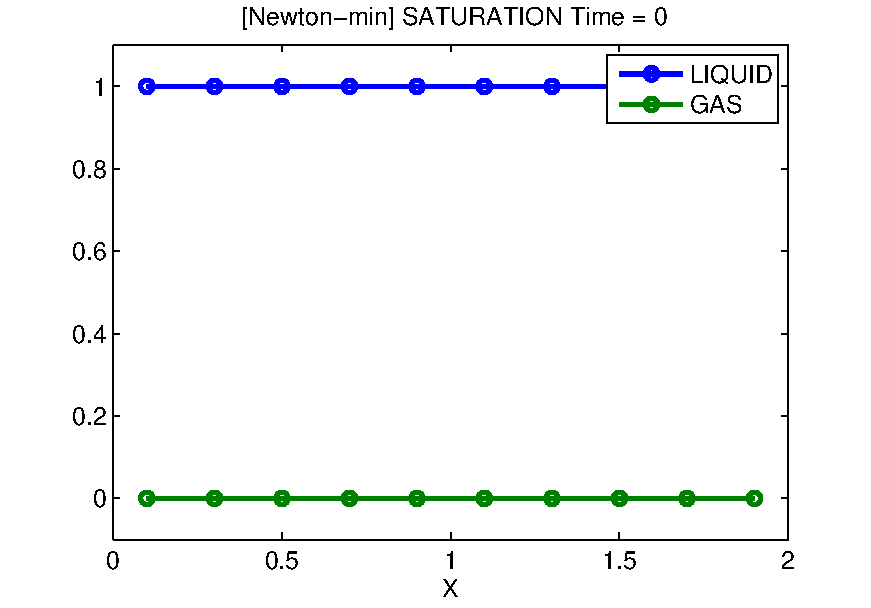
\includegraphics[scale=0.30]{saturation_initiale}   & 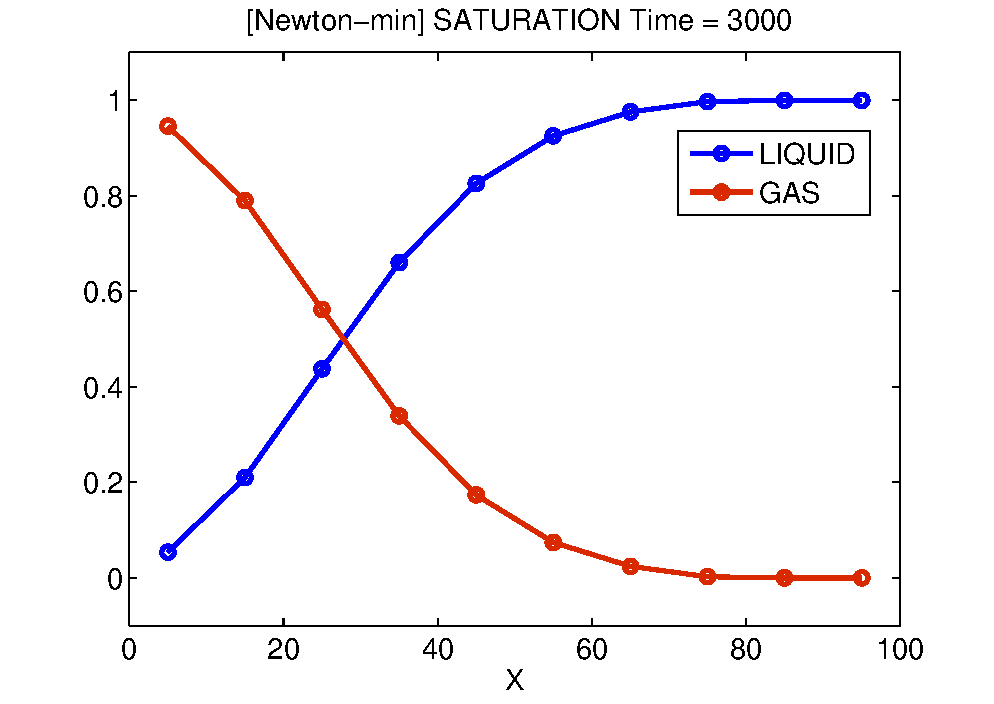
\includegraphics[scale=0.28]{saturation_3000} \\
%   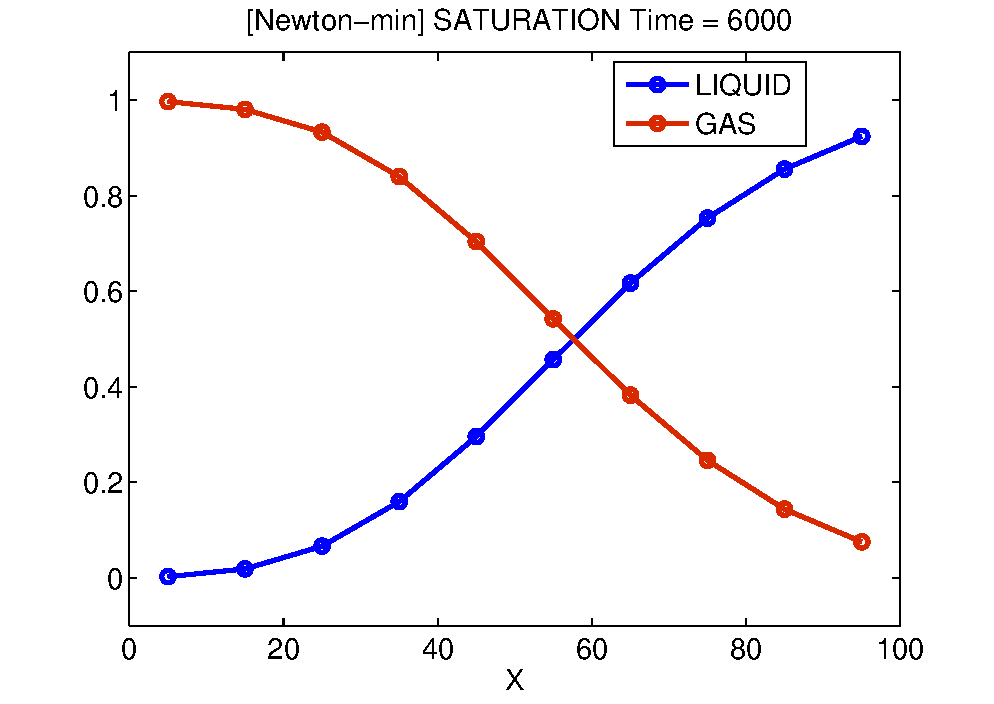
\includegraphics[scale=0.29]{saturation_6000} & 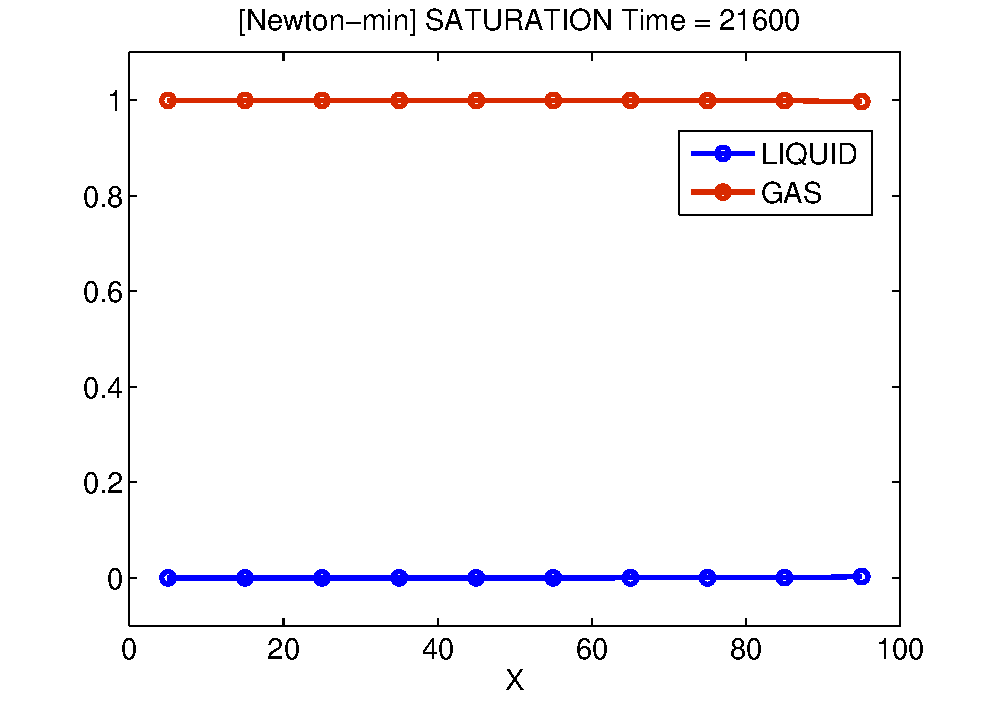
\includegraphics[scale=0.29]{saturation_21600}  \\
%\end{tabular}
%\end{frame}
\section{Conclusion}
\begin{frame}
\frametitle{Conclusion}
\begin{itemize}
\item[$\bullet$] Problème des membranes: Extension de mes travaux à la méthode de Newton--min inexacte tenant compte du solveur algébrique linéaire multigrille. Construire un estimateur d'erreur a posteriori entre la solution exacte $\bu$ et la solution approchée linéarisée algébrique $\uhki$, critère d'arrêt.
\textcolor{red}{Extension du Théorème \eqref{eq: a_posteriori_membrane}  au cas où $\lambda_h \ngeq 0$.} Simulation numérique.
\vspace{1 cm}
\item[$\bullet$] Problème diphasique liquide--gaz:
Construction d'un estimateur d'erreur a posteriori, critère d'arrêt: Newton--min adaptatif.
\end{itemize}
\end{frame}
\begin{frame}
\begin{center}
{\Large \textbf {Merci pour votre attention}}
\end{center}
\end{frame}
\bibliographystyle{plain}
\bibliography{biblio}
\end{document}
